
\begin{figure}[t]
    \centering
    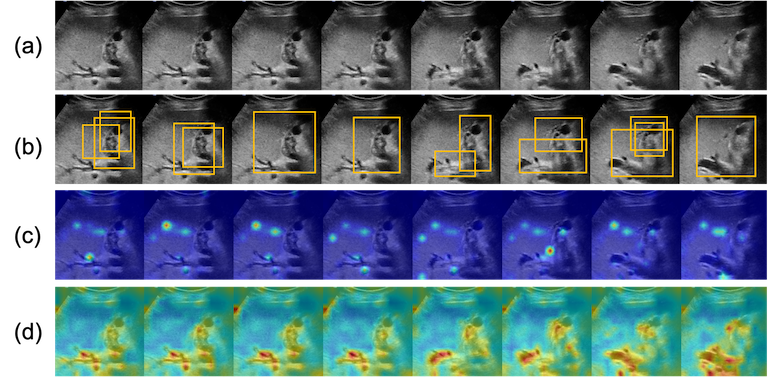
\includegraphics[width=\linewidth]{figs/vis_gbc_focusmae.png}
    \caption[Visual demonstration of the benefit of using the \focusmae]{Visual demonstration of the benefit of using the \focusmae method for GBC detection. (a) Original frames from a USG video sequence exhibiting GB malignancy. (b) Candidate regions as prior (in yellow). (d), (e) Attention visualization for the downstream malignancy detection for VideoMAE and \focusmae, respectively. For \focusmae, the attention is well guided to the key regions containing the malignancy, as opposed to VideoMAE.}
    \label{focusmae_fig:qualitative}
\end{figure}

\begin{figure}[!ht]
    \centering
    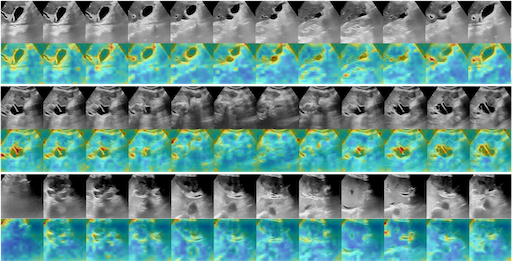
\includegraphics[width=\linewidth]{figs/vis_attention_gbc.png}
    \caption[Attention visuals for \focusmae for GBC detection]{Attention visuals for \focusmae for the GBC detection task on the USG videos. We show three different maligant video samples. For each video sample, the upper row shows the sequence with the original frames, and the lower row shows the attention on the frames.}
    \label{focusmae_fig:visual_supp_gbc}
\end{figure}

\section{Experiments and Results}
%
\subsection{Efficacy of \focusmae over SOTA Baselines}
%
We explore the GBC classification performance on USG videos for five SOTA video classification methods, namely Video-Swin \cite{videoswin}, TimeSformer \cite{timesformer}, VidTr \cite{vidtr}, VideoMAEv2 \cite{videomaev2}, and AdaMAE \cite{adamae}. 

In addition, we have also explored our previously developed SOTA techniques \cite{basu2022surpassing, basu2023radformer, basu2022unsupervised} that are specialized for GBC detection on USG images. Apart from these specialized models, we analyze the performances of popular image-centric CNN-based classifiers \cite{resnet,inception} and detectors \cite{fasterrcnn, efficientdet}. We also look into three popular Transformer-based classifiers - ViT \cite{vit}, DEiT \cite{touvron2021training}, and PvT \cite{wang2021pvtv2} for GBC detection. 


\mypara{Using Image-based Methods for Video Classification}
%
We use the same video sub-sampling scheme used during the fine-tuning phase (ref. \cref{label:impl_ft}) of the \focusmae to get the frames and clips. We then use the image-centric methods to predict the labels for each frame in the clips. If the majority of the frames in a clip are predicted as malignant, then the clip is predicted as malignant. If any clip within a video is predicted as malignant, the overall video is categorized as malignant. The image-based methods were pretrained on the public GBCU \cite{basu2022surpassing} dataset. 

\mypara{Quantitative Analysis}
%
We show the 5-fold cross-validation performance in terms of accuracy, specificity, and sensitivity for the baselines and the proposed \focusmae in \cref{tab:main}. Clearly, the video-based techniques trump the image-centric SOTA methods of GBC detection, supporting our recommendation of a paradigm shift to video-based classification for the problem. Additionally, we see the effectiveness of the \focusmae in detecting GBC. 


\mypara{Qualitative Analysis}
%
We show the qualitative analysis in \cref{focusmae_fig:qualitative}. The random masking by VideoMAE does not adequately mask the high-information malignant region. In contrast, the region prior guided \focusmae generates stronger masking for learning the malignant representation by biasing the masking towards the malignancy localization region. We visualize the attention rollout during the downstream task. Clearly, \focusmae's attention regions highlight semantically more meaningful areas, such as the gallbladder boundary and anatomical structures, compared to VideoMAE. More visuals for FocusMAE attention is shown in \cref{focusmae_fig:visual_supp_gbc}.

\subsection{Generality of the Proposed Method}
%
\begin{table}[!t]
    \footnotesize
	\centering
	%\resizebox{ \linewidth}{!}{%
	\begin{tabular}{llccc}
		\toprule
		{\textbf{Group}} & {\textbf{Method}} & {\textbf{Acc.}} &  {\textbf{Spec.}} & {\textbf{Sens.}} \\
		\midrule
		%
		\multirow{5}{*}{Image-based} 
		& ResNet50 \cite{resnet} & 0.721 & 0.739 & 0.711 \\
		%
		& InceptionV3 \cite{inception} & 0.672 & 0.739 & 0.632 \\
        %
        %& USG-UCL \cite{basu2022unsupervised} & 0.802 & 0.869 & 0.763\\
		%
        \cmidrule{2-5}
        & ViT \cite{vit} & 0.770 & 0.783 & 0.763 \\
		%
		& DEIT \cite{touvron2021training} & 0.770 & 0.696 & 0.816 \\
		%
		\midrule
		\multirow{3}{*}{Video-based} 
        %& ViViT \cite{vivit} & Transformer & & & \\
		%
        %& Video-Swin \cite{videoswin} & 0.820 & 0.695 & 0.894 \\
		%
        & TimeSformer \cite{timesformer} & 0.787 & 0.739 & 0.816 \\
        %
        %& VidTr \cite{vidtr} & 0.443 & 0.826 & 0.210 \\
		%
		& VideoMAE \cite{videomae} & 0.852 & 0.956 & 0.789 \\
		%
		%& AdaMAE \cite{adamae} & & & \\
		%
		\cmidrule{2-5}
		& FocusMAE (Ours) & 0.885 & 0.895 & 0.869 \\
		\bottomrule
	\end{tabular}
	%}
	\caption[Comparison of SOTA and \focusmae for Covid detection]{The performance comparison in terms of accuracy, specificity, and sensitivity of baselines and \focusmae for detecting COVID from CT \cite{covidctmd}. CT-slices are analogous to the video frames, and thus, video-based detection methods are applicable to CT modality as well. Our proposed method consistently outperforms the SOTA baselines on the COVID detection task, establishing the generality and applicability of our method across two different medical imaging modalities - USG and CT. }
	\label{tab:covid}
\end{table}



\begin{figure}[!t]
    \centering
    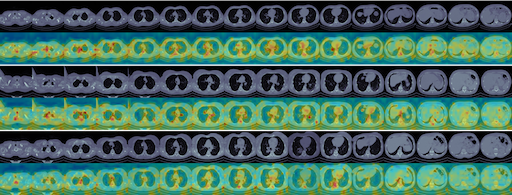
\includegraphics[width=\linewidth]{figs/vis_attn_covid.png}
    \caption[Attention visuals for \focusmae for Covid detection]{Attention visuals for \focusmae for COVID detection from CT images. We show four COVID CT samples. For each  sample, the upper row shows the sequence with the original CT slices, and the lower row shows the attention on these slices.}
    \label{focusmae_fig:visual_supp_covid}
\end{figure}

%
We explored the generality of the proposed \focusmae method on the task of Covid detection from a publicly available CT dataset \cite{covidctmd}. \cref{tab:covid} shows that \focusmae achieves much better accuracy, specificity, and sensitivity, indicating the superiority of the disease representation learning capability of \focusmae. \cref{focusmae_fig:visual_supp_covid} shows the attention visuals for COVID detection. The applicability of \focusmae on two distinct tasks -- 1) GBC detection from USG videos, and 2) Covid detection from CT -- provides evidence of generality of the method. 


\subsection{Ablation Study}
\begin{figure}[!t]
	\centering
	\begin{subfigure}[b]{0.23\linewidth}
        \centering
        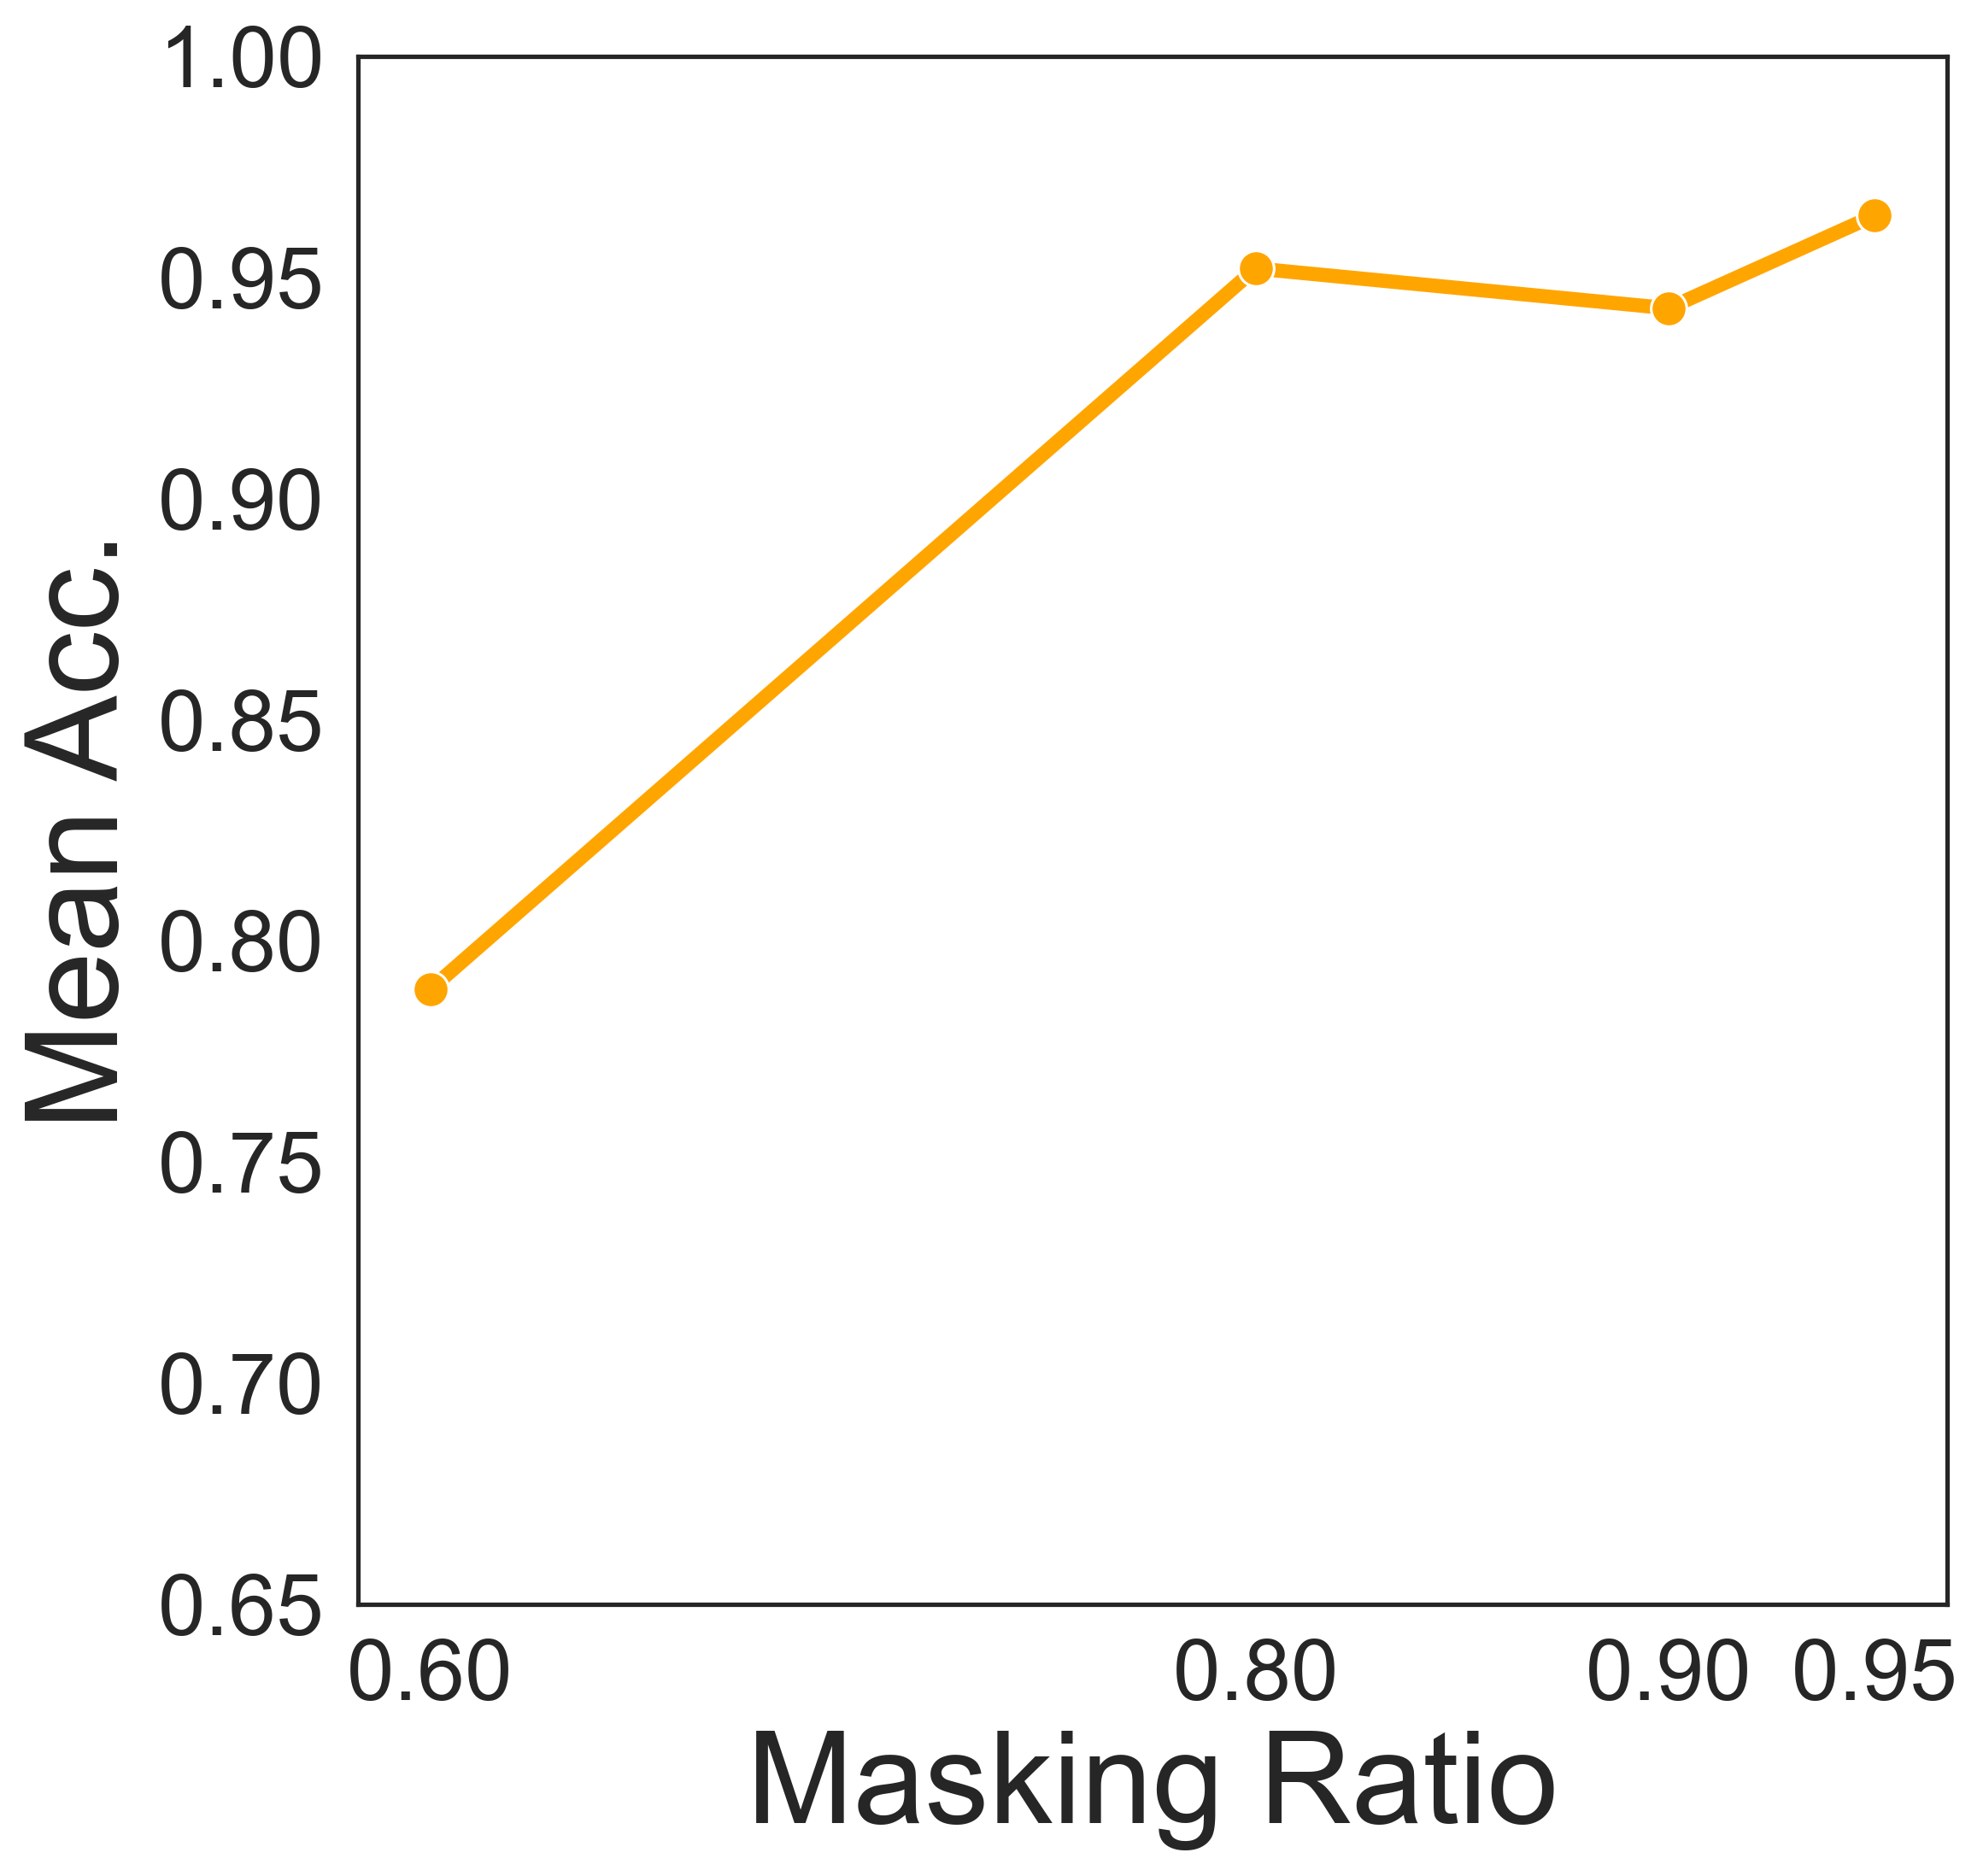
\includegraphics[width=\linewidth]{figs/focusmae/abl_mr.png}
        \caption{}
        \label{focusmae_fig:ablation_mr}
    \end{subfigure}
	\begin{subfigure}[b]{0.23\linewidth}
		\centering
		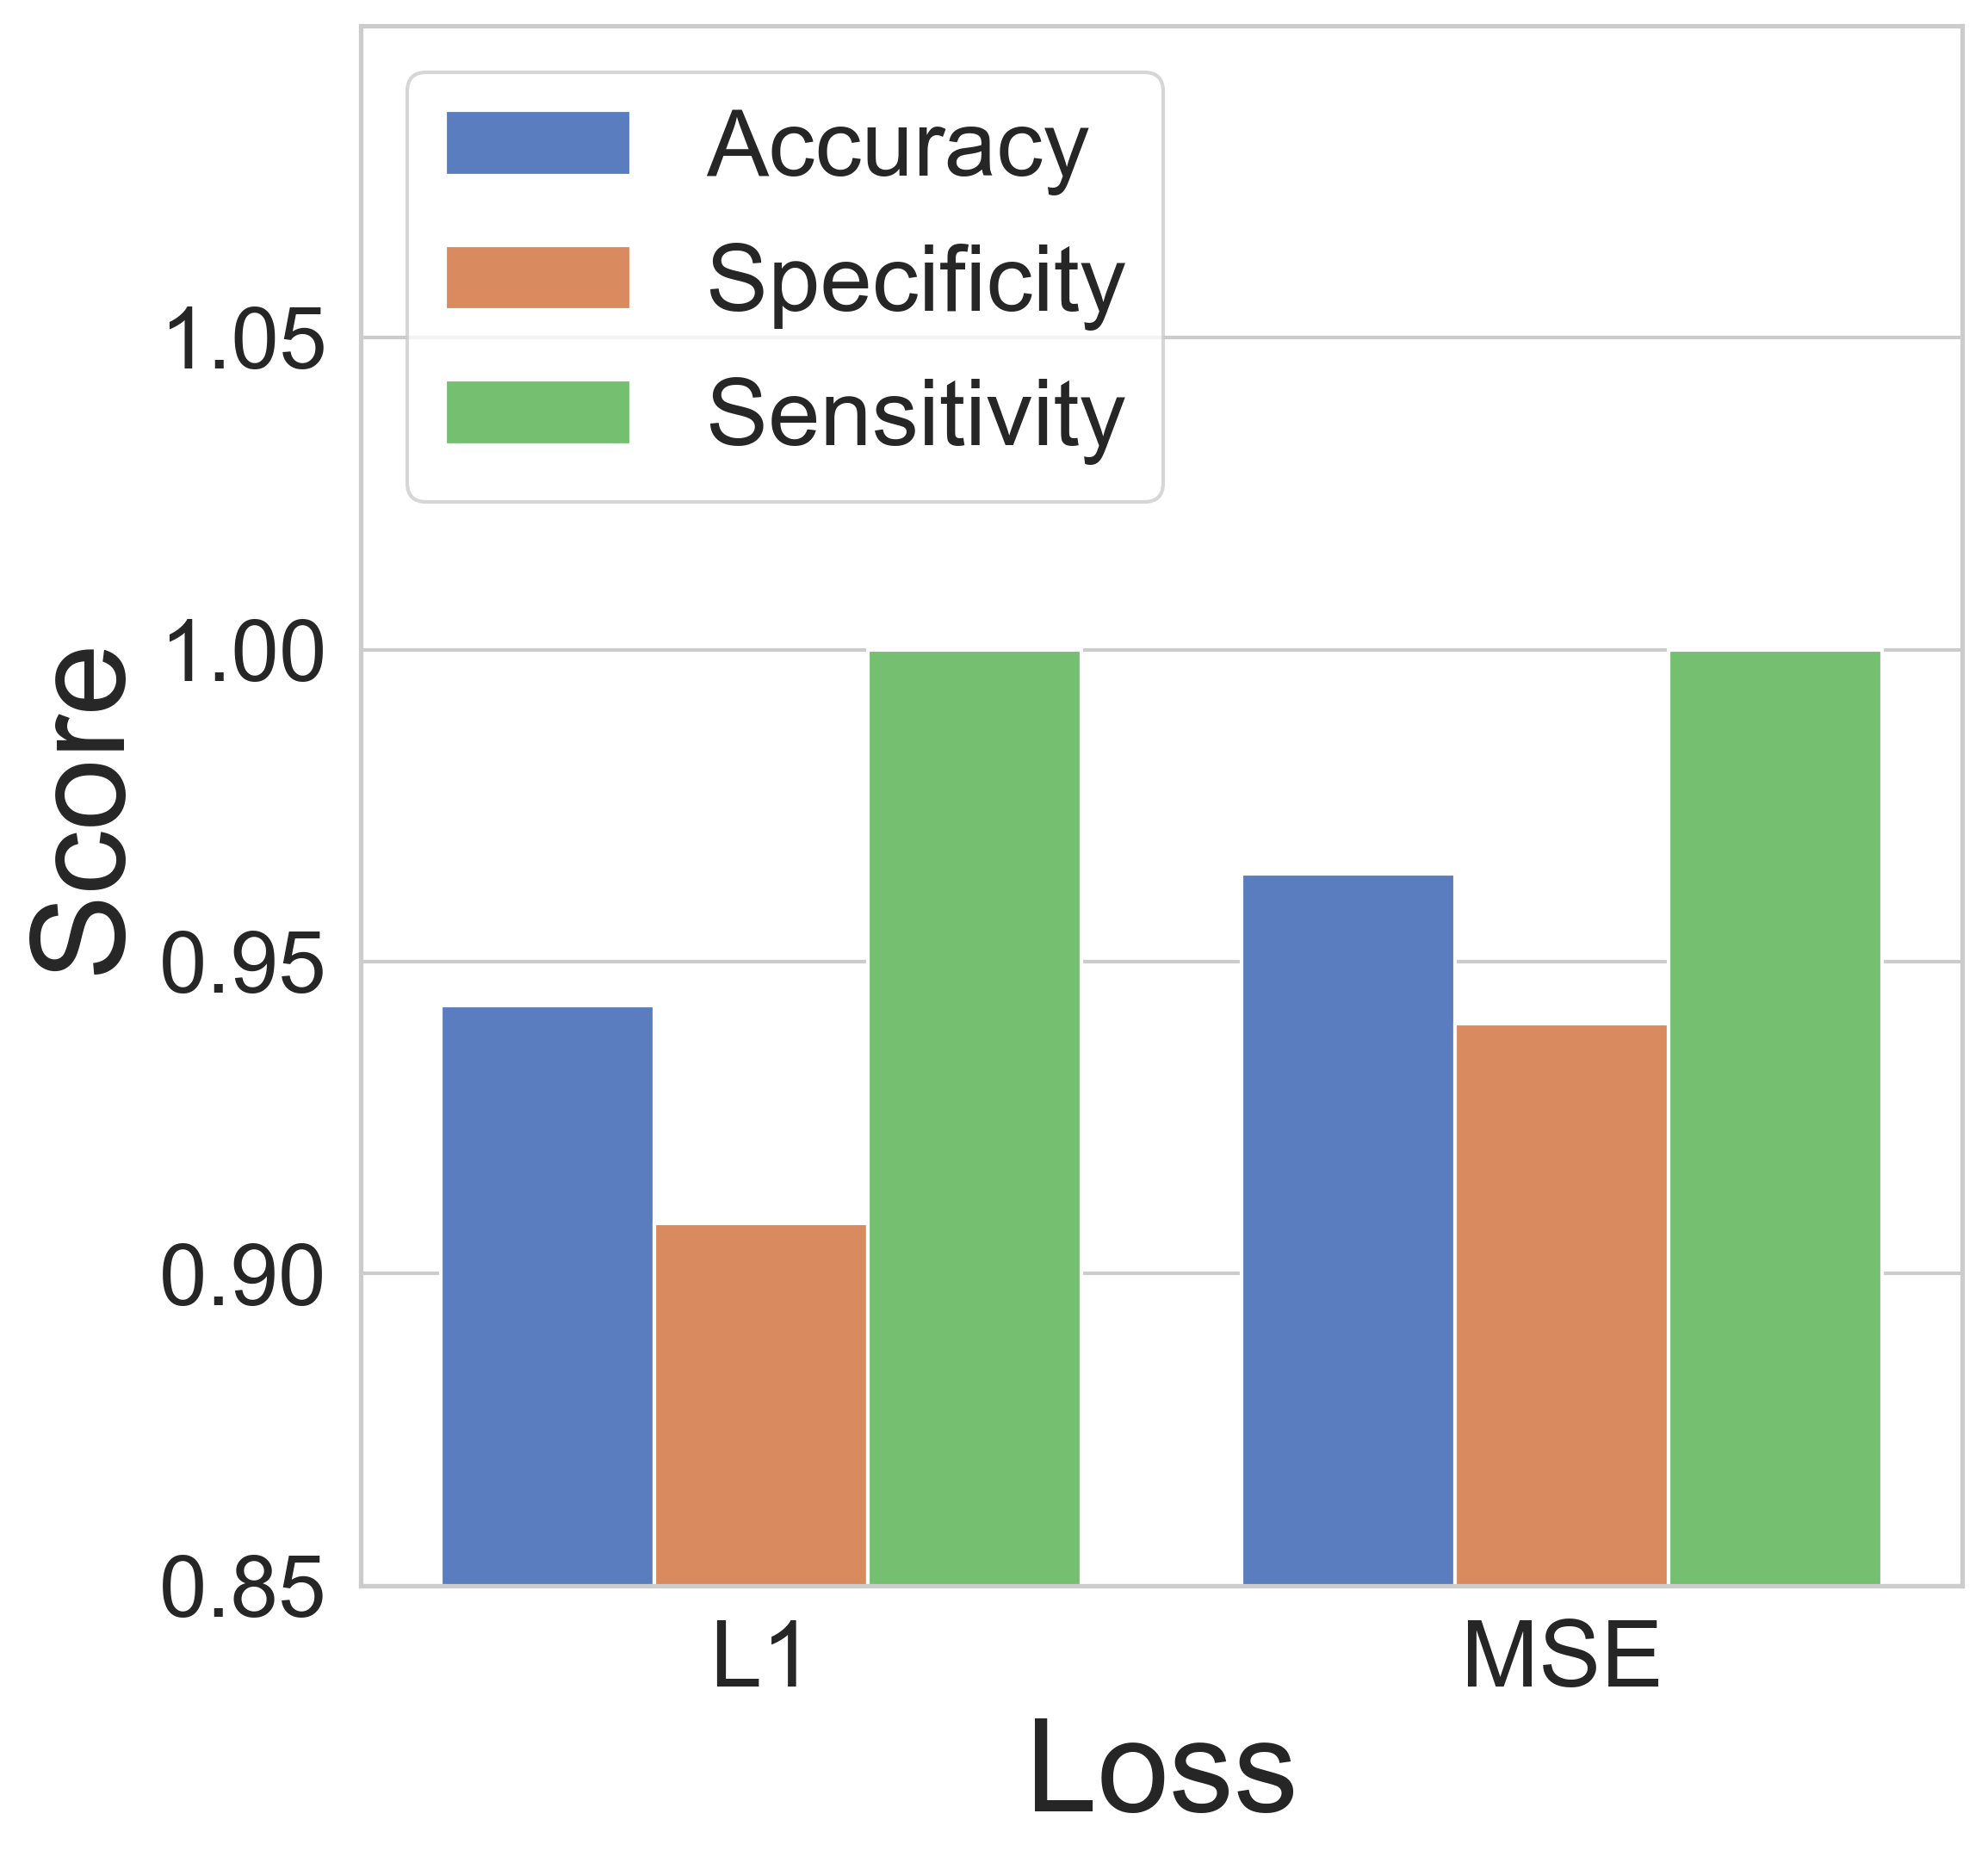
\includegraphics[width=\linewidth]{figs/focusmae/abl_loss.png}
		\caption{}
		\label{focusmae_fig:ablation_loss}
	\end{subfigure}
 %
	\begin{subfigure}[b]{0.23\linewidth}
		\centering
		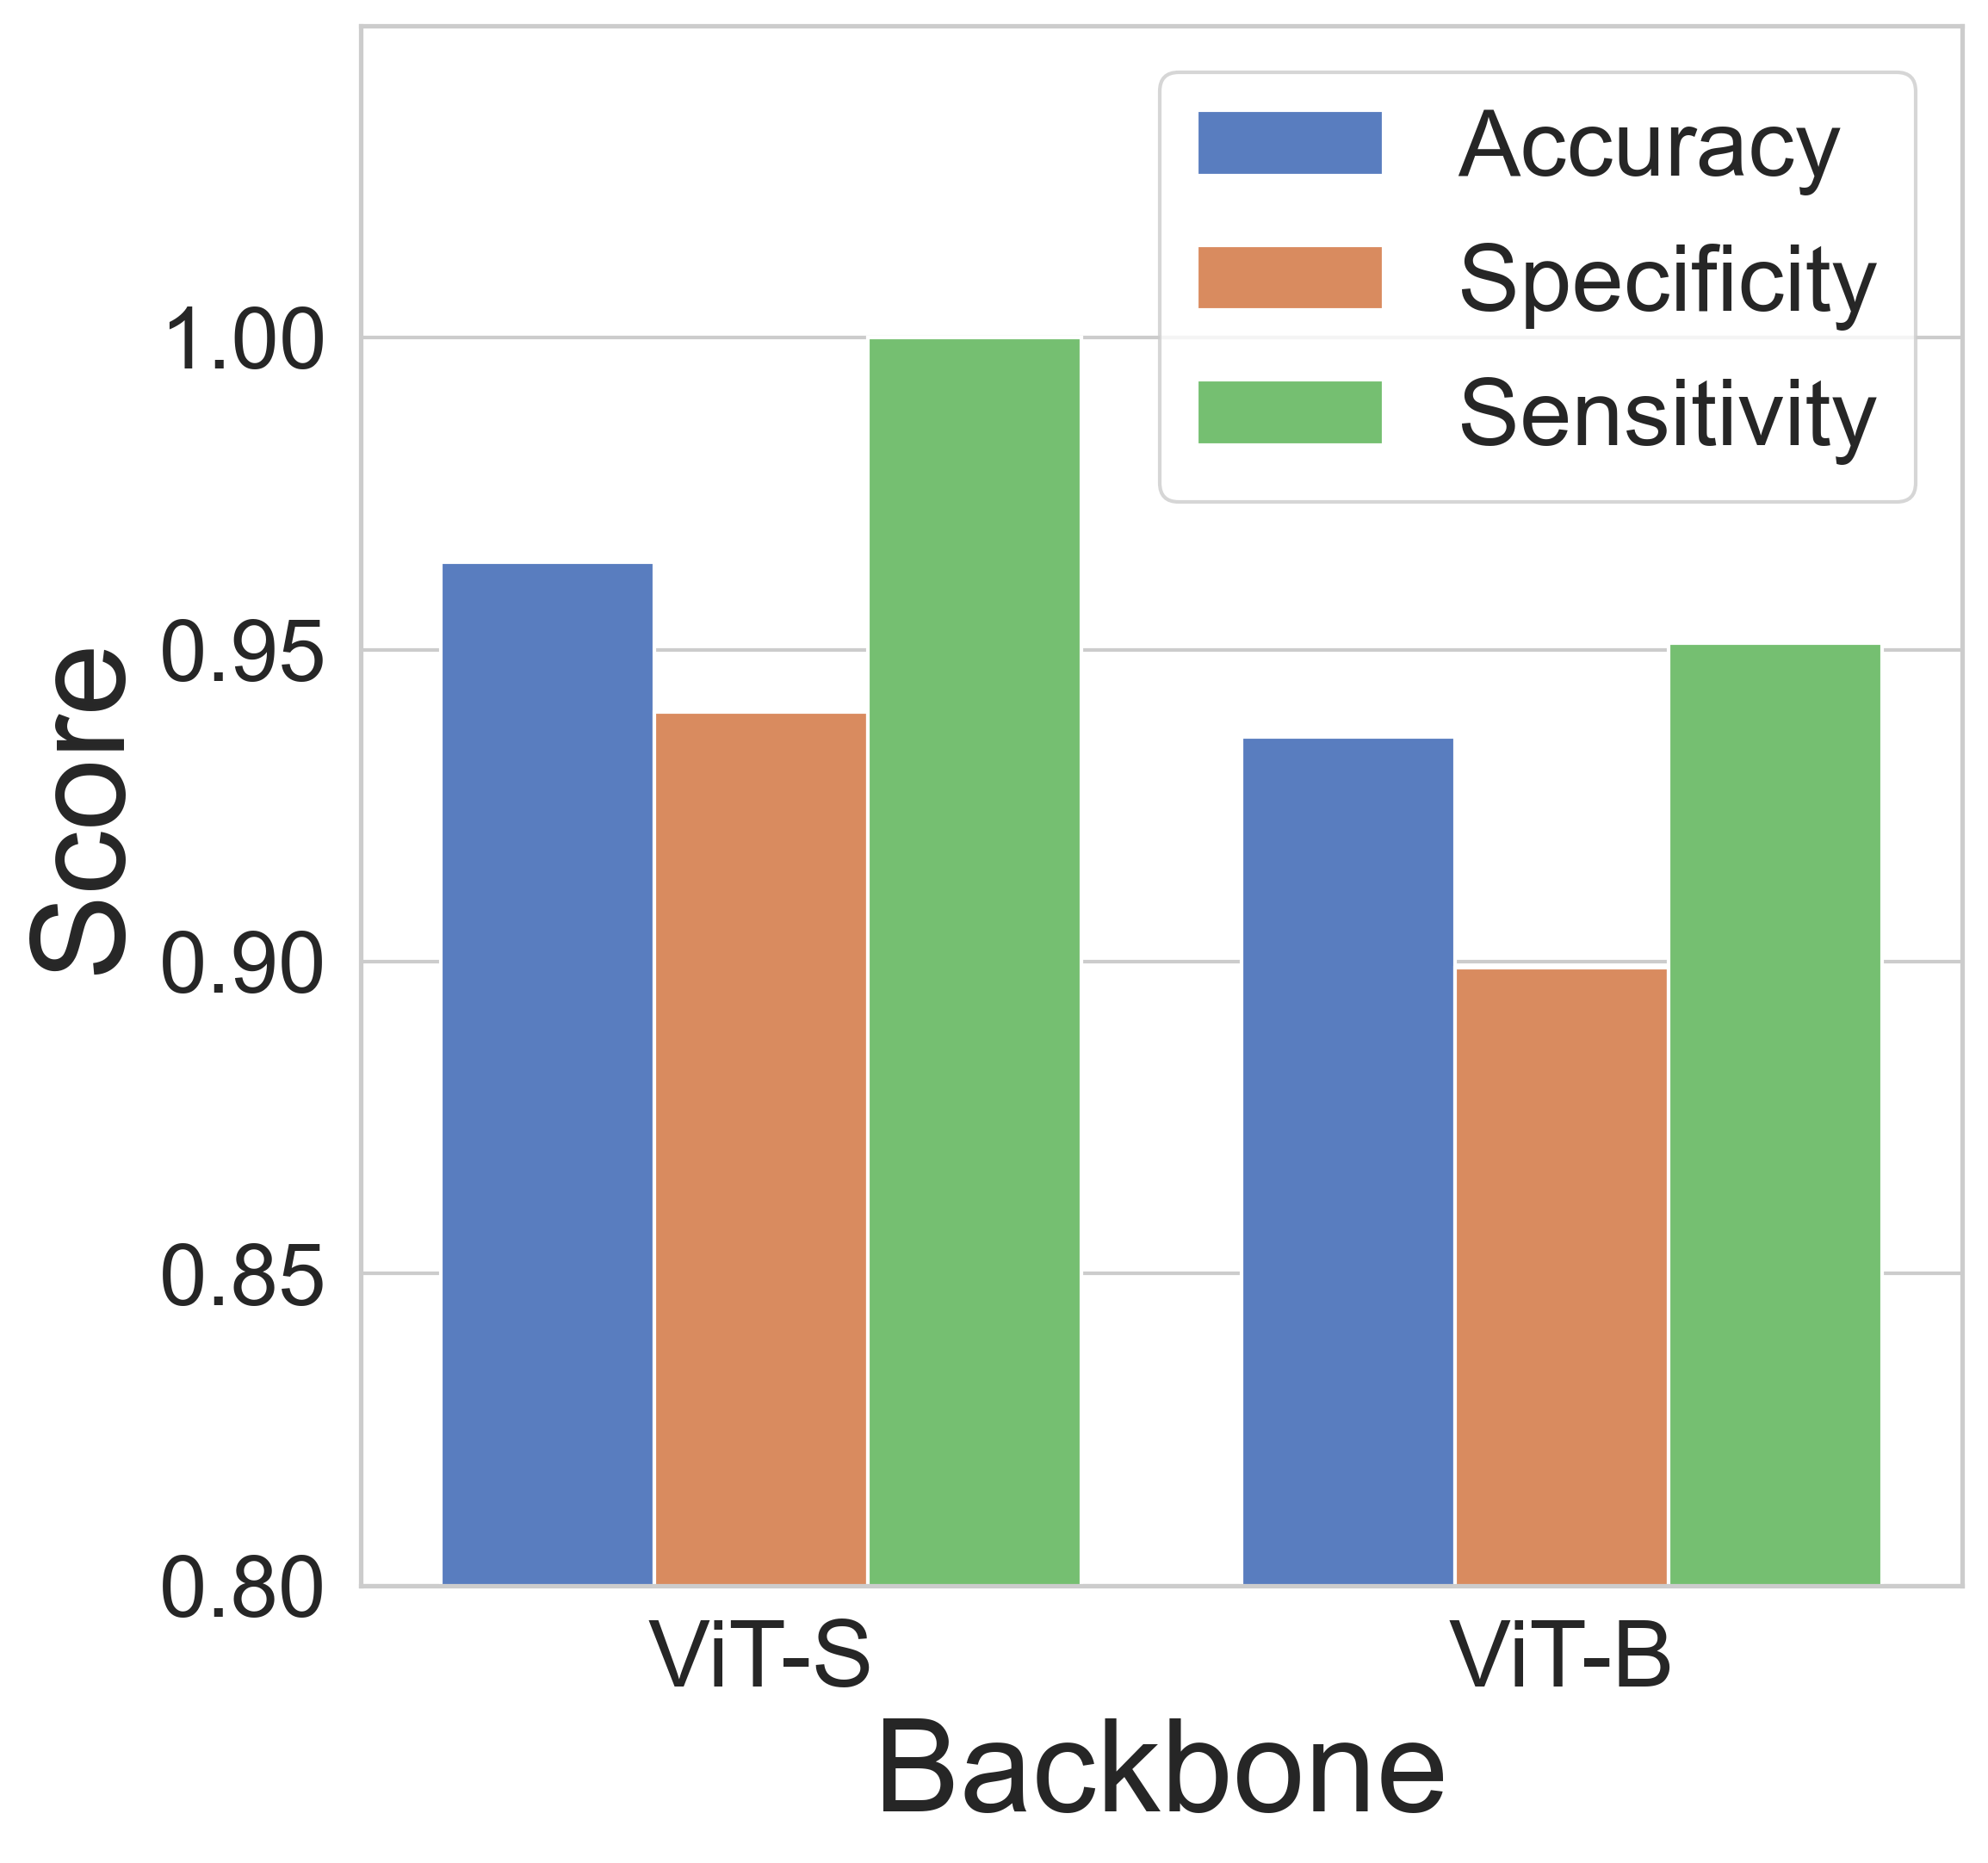
\includegraphics[width=\linewidth]{figs/focusmae/abl_enc.png}
		\caption{}
		\label{focusmae_fig:ablation_enc}
    \end{subfigure}	
    \begin{subfigure}[b]{0.23\linewidth}
		\centering
		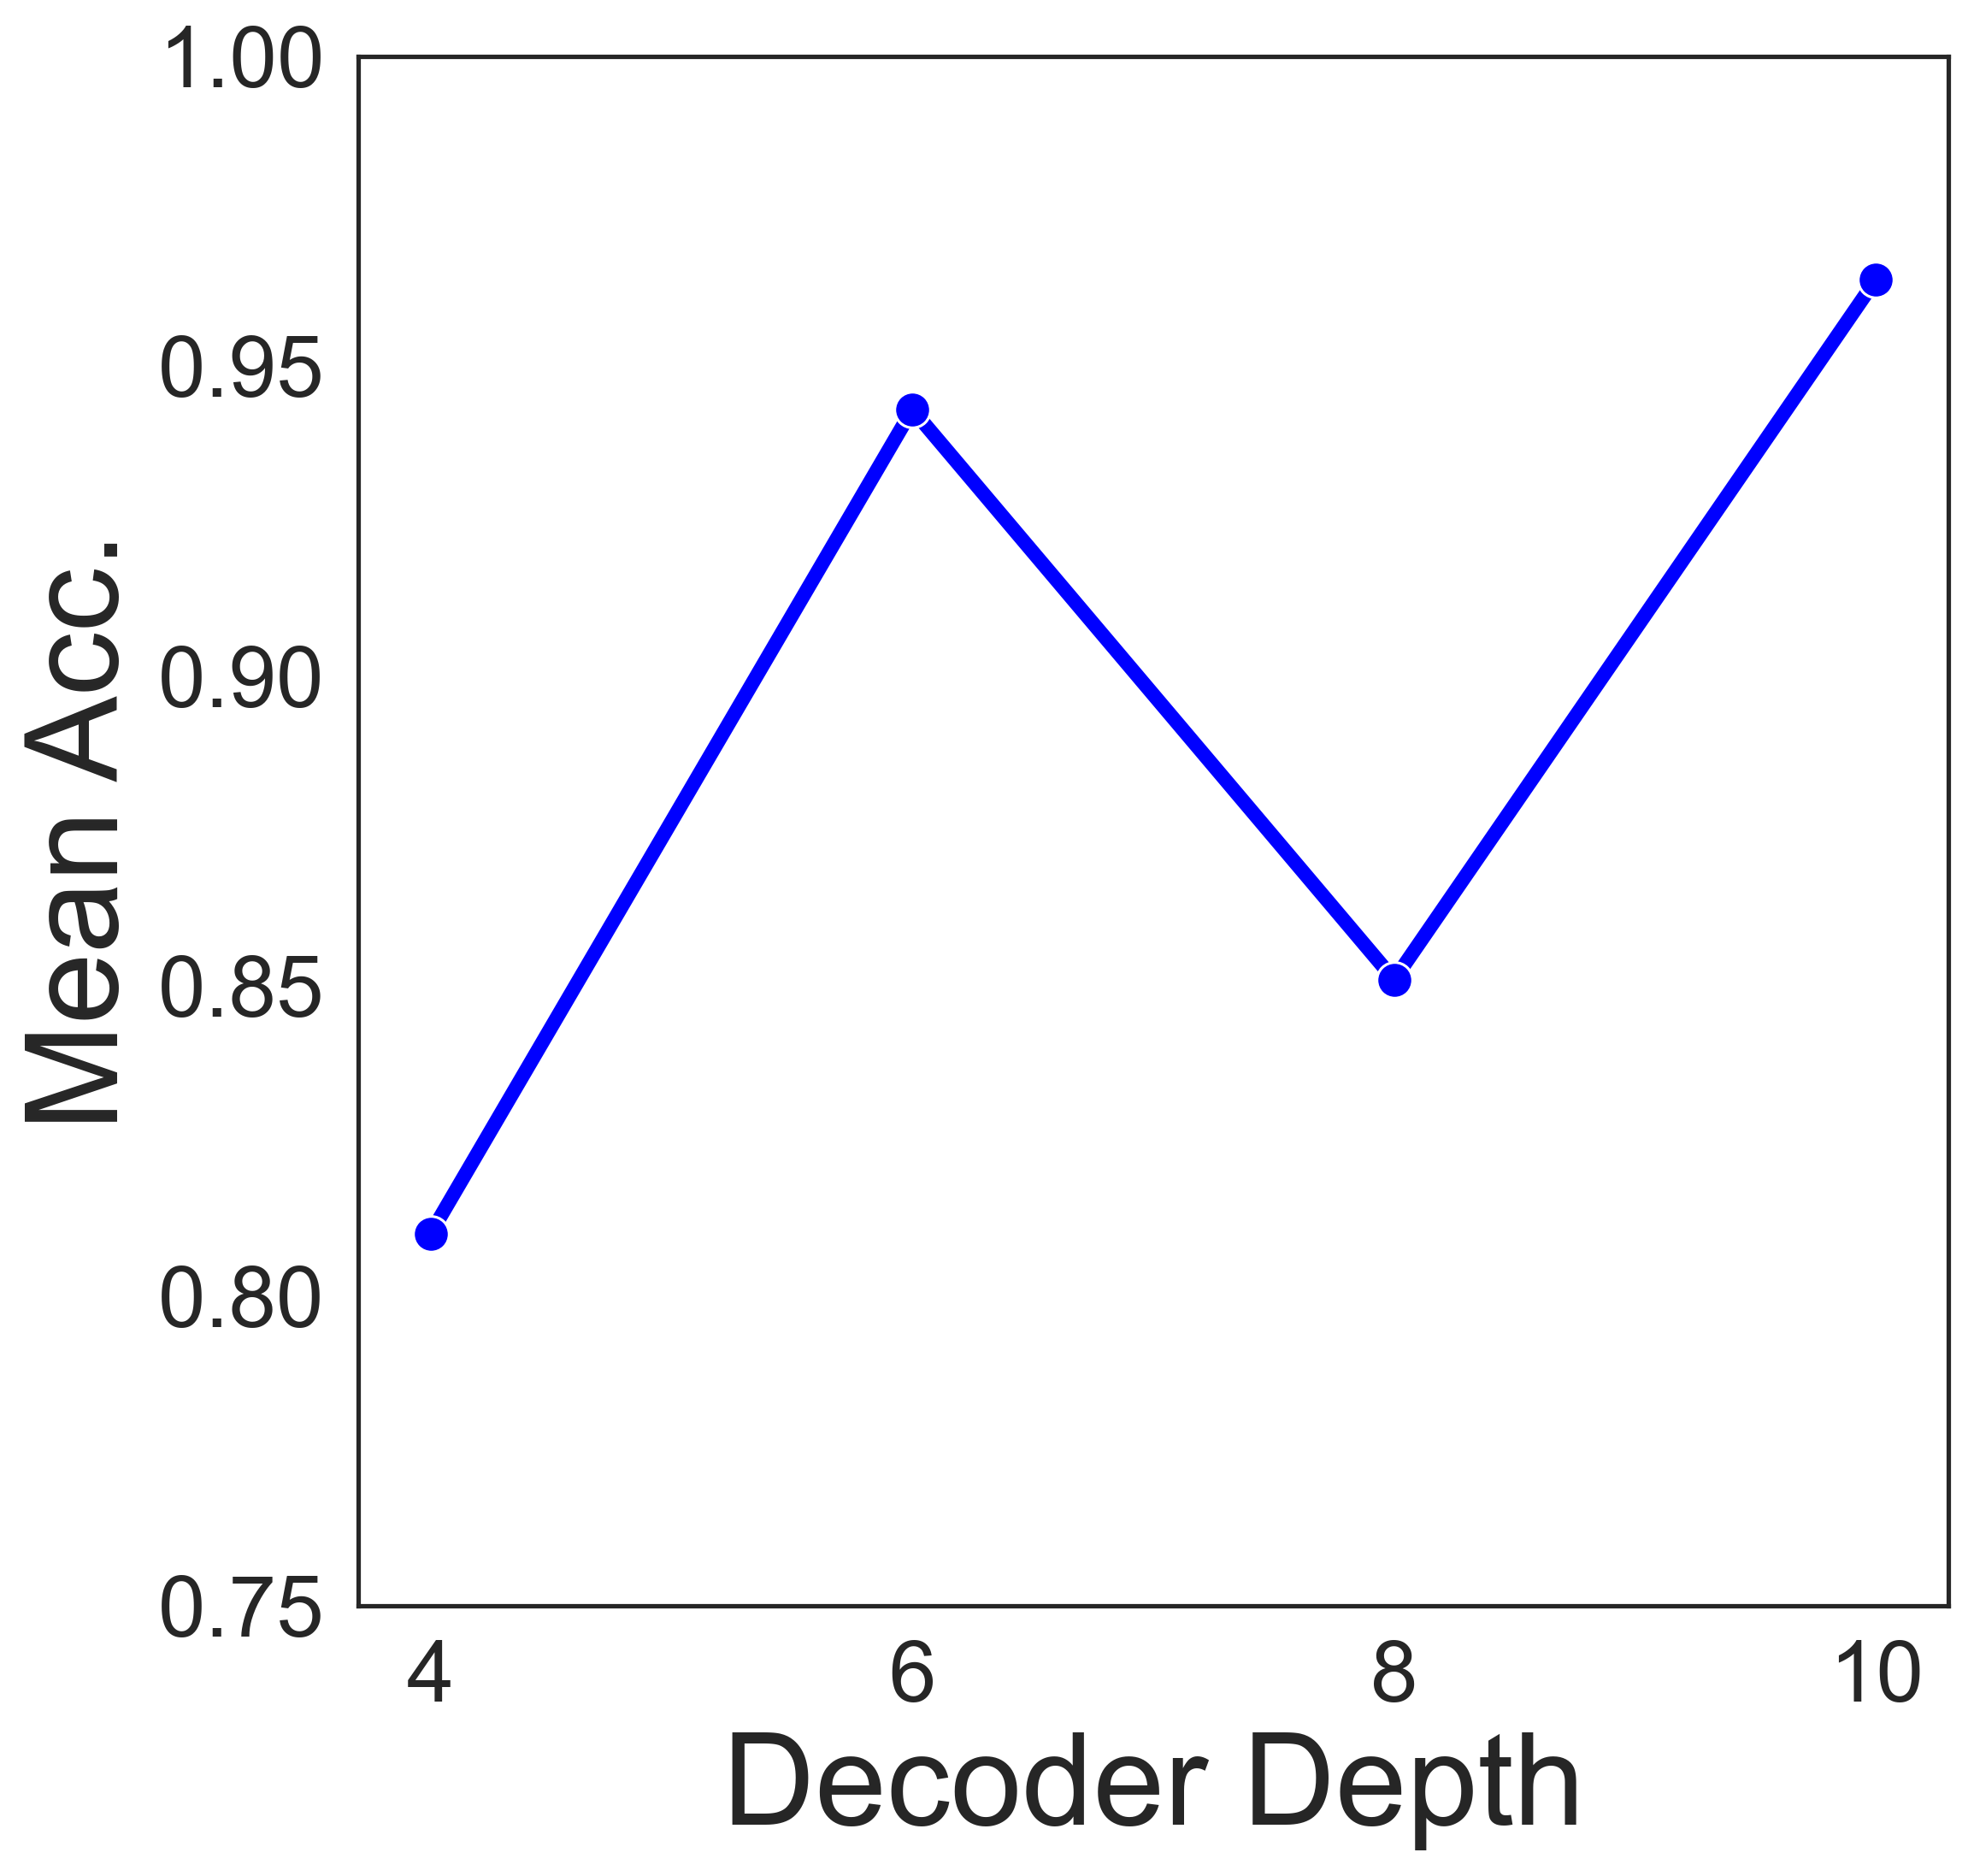
\includegraphics[width=\linewidth]{figs/focusmae/abl_dec.png}
		\caption{}
		\label{focusmae_fig:ablation_dec}
	\end{subfigure}
	\caption[Ablation study on \focusmae]{Ablation study. We report the mean scores over 5-fold cross-validation for GBC detection. (a) Effect of varying the masking ratio ($\rho$) on accuracy. (b) Effect of varying the reconstruction loss - L1 vs. MSE - for SSL pretraining. Training with MSE yields 2.2\% better accuracy. (c) Performance for different backbones. (d) Effect of varying the decoder depth on the accuracy. }
	\label{focusmae_fig:ablation}
\end{figure}

\begin{table}[!t]
	\centering
    \footnotesize
	\resizebox{ \linewidth}{!}{%
	\begin{tabular}{cccccccc}
		\toprule
		\multirow{3}{*}{\textbf{Masking Ratio}} & \multirow{3}{*}{\textbf{Decoder Depth}} & \multicolumn{6}{c}{\textbf{Loss}} \\
        & & \multicolumn{3}{c}{\textbf{MSE}} & \multicolumn{3}{c}{\textbf{L1}} \\
        & & Acc. & Spec. & Sens. & Acc. & Spec. & Sens. \\
        %& {\textbf{Time/Frame (ms)}}\\
		\midrule
		%
        \multirow{4}{*}{0.6}
		& 4  & 0.538$\pm$0.443 & 0.808$\pm $0.123& 0.940$\pm$0.120 & 0.943$\pm$0.065 
         & 0.940$\pm$0.120 & 0.938$\pm$0.076 \\
  
        & 6 & 0.952$\pm$0.071 & 0.940$\pm$0.120 & 1.000$\pm$0.000 & 0.943$\pm$0.065& 0.940$\pm$0.120& 0.938$\pm$0.076  \\
        
        & 8 & 0.942$\pm$0.066 & 0.940$\pm$0.120 & 0.938$\pm$0.076& 0.943$\pm$0.065 & 0.940$\pm$0.120 & 0.938$\pm$0.076  \\
        
        & 10 & 0.749$\pm$0.144 & 0.940$\pm$0.120 & 0.600$\pm$0.490  & 0.943$\pm$0.065 & 0.940$\pm$0.120 & 0.938$\pm$0.076  \\
		%
        \midrule 
        %
		\multirow{4}{*}{0.8}
		& 4 & 0.940$\pm$0.066  & 0.940$\pm$0.120& 0.938$\pm$0.076 & 0.86$\pm$0.124 & 0.699$\pm$0.371 & 0.940$\pm$0.120 \\
        & 6 & 0.942$\pm$0.065  & 0.940$\pm$0.120 & 0.938$\pm$0.076 & 0.943$\pm$0.065 & 1.000$\pm$0.000 & 0.938$\pm$0.076 \\
        & 8 & 0.942$\pm$0.066 & 0.940$\pm$0.120 & 0.938$\pm$0.076 & 0.978$\pm$0.027 & 1.000$\pm$0.000 & 0.938$\pm$0.076\\
        & 10 & 0.952$\pm$0.070 & 0.940$\pm$0.120 & 0.967$\pm$0.067 & 0.943$\pm$0.065 & 0.940$\pm$0.120 & 0.938$\pm$0.076 \\
		%
        \midrule 
        %
        \multirow{4}{*}{0.95}
		& 4 & 0.810$\pm$0.124 &0.940$\pm$0.120& 0.538$\pm$0.443 & 0.943$\pm$0.065 &0.940$\pm$0.120 & 0.938$\pm$0.076 \\
        & 6 & 0.943$\pm$0.065 & 0.940$\pm$0.120 & 0.938$\pm$0.076& 0.943$\pm$0.065 & 0.940$\pm$0.120 & 0.938$\pm$0.076 \\
        & 8 & 0.811$\pm$0.122&0.940$\pm$0.120 & 0.538$\pm$0.443 & 0.943$\pm$0.065 & 0.940$\pm$0.120 & 0.938$\pm$0.076 \\
        & 10 & 0.964$\pm$0.072 & 0.940$\pm$0.120 & 1.000$\pm$0.000 & 0.943$\pm$0.065& 0.940$\pm$0.120 & 0.938$\pm$0.076 \\
		%
  %       \midrule 
  %       %
  %       \multirow{4}{*}{1}
		% & 4 & 0.966$\pm$0.028 & 1.000$\pm$0.000 & 0.909$\pm$0.074 & 0.965$\pm$0.071 & 0.940$\pm$0.120 & 1.000$\pm$0.000 \\
  %       & 6 & 0.943$\pm$0.065 & 0.940$\pm$0.120& 0.938$\pm$0.076 &0.943$\pm$0.065 &1.000$\pm$0.000 &0.938$\pm$0.076  \\
  %       & 8 & 0.943$\pm$0.065 & 0.940$\pm$0.120 & 0.938$\pm$0.076 & 0.943$\pm$0.065 &1.000$\pm$0.000 &0.938$\pm$0.076  \\
  %       & 10 & 0.966$\pm$0.028 & 1.000$\pm$0.000 & 0.91$\pm$0.074 & 0.943$\pm$0.065 &1.000$\pm$0.000 &0.938$\pm$0.076 \\
		\bottomrule
	\end{tabular}
	}
	\caption[Hyperparameter tuning of \focusmae]{Hyperparameter tuning. We vary the Masking ratio, Decoder depth, and the loss function for a grid search. We report the 5-fold cross-validation (Mean$\pm$SD) accuracy, specificity, and sensitivity for \focusmae in detecting GBC from the USG.}
	\label{focusmae_tab:hyperparam_supp}
\end{table}


%
We performed the ablation study on the FocusMAE with the ViT backbone on the USG Video dataset. We show the mean scores over the 5-fold cross-validation.

\mypara{Masking Ratio}
%
\cref{focusmae_fig:ablation_mr} shows how the masking ratio $\rho$ influences the performance of \focusmae. For \focusmae, 95\% masking ratio achieves the best accuracy of 96.4\%. VideoMAE uses a 90\% masking ratio with random tube-based masking. The region-prior guided approach helps \focusmae to sample more informative tokens with lower redundancy than VideoMAE.

\mypara{Reconstruction Loss}
%
We examined the effect of varying the reconstruction loss function in our study. We experimented with two variants: Mean Absolute Error or L1-loss, and Mean Squared Error (MSE). The results, shown in \cref{focusmae_fig:ablation_loss}, indicate that using MSE loss during pretraining produces better performance in terms of accuracy. Models trained with MSE loss demonstrated a 2.2\% higher mean accuracy compared to those trained with L1 loss.

\mypara{Encoder Backbone}
%
\cref{focusmae_fig:ablation_enc} demonstrates the effect of ViT variants on the token encoding task. We experimented with ViT-S and ViT-B. We observe that larger backbones do not perform well for our data, indicating potential over-fitting.

\mypara{Decoder Depth}
%
We experiment with the number of decoder blocks and present the result in \cref{focusmae_fig:ablation_dec}. We see performance gain when the decoder depth is varied from 4 to 6. However, there is a drop in performance when the decoder depth is increased to 8. The observation is consistent with \cite{videomae, adamae}. Interestingly, when we increased the depth further, we saw an increase in accuracy, which indicates that the decoder can benefit from increasing the depth and need not necessarily be a shallow network. 

\mypara{Hyper-parameter Selection}
%
We performed a rigorous grid search for selecting the hyper-parameters. \Cref{focusmae_tab:hyperparam_supp} shows the grid search result.  

\begin{figure}[t]
    \centering
    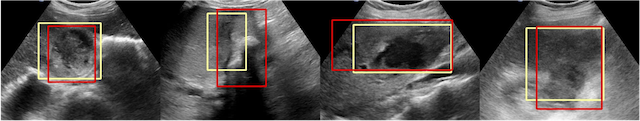
\includegraphics[width=\linewidth]{figs/focusmae/roi_vis.png}
    \caption[Visuals of candidate region priors]{Visuals of candidate regions. Red -- malignant regions identified by radiologists. Yellow -- candidate object localization generated by the RPN.}
    \label{focusmae_fig:roi}
\end{figure}

\subsection{Analysis on Candidate Region Selection}
\cref{focusmae_fig:roi} shows sample object region localization of the RPN. We adopted a FasterRCNN-based RPN for generating the candidate regions for using as priors in \focusmae. We used the GBCU dataset to pretrain the detectors for localizing the malignancy. We then lowered the threshold to generate multiple candidate regions for the video frames used in the \focusmae experiments. To calculate precision and recall in the GB localization phase, following the recommendation of \cite{ribli2018detecting}, we determine a predicted bounding box region as a true positive if its center falls within the the ground truth bounding box region. Conversely, if the center is outside the bounding box, we categorize the prediction as a false positive attributed to localization error. The RPN achieves mIoU of 0.712 with a recall rate of 0.994.